\documentclass[11pt]{article}

\usepackage[a4paper,margin=1in]{geometry}
\usepackage{amsmath}
\usepackage{amssymb}
\usepackage{booktabs}
\usepackage{float}
\usepackage{graphicx}
\usepackage{longtable}
\usepackage{pdflscape}
\usepackage{tabularx}
\usepackage{tikz}
\usetikzlibrary{arrows.meta,positioning}
\usepackage{caption}
\usepackage{subcaption}
\usepackage[hidelinks]{hyperref}
\usepackage[authoryear,round]{natbib}
\usepackage{siunitx}
\sisetup{group-digits=integer,group-separator={,},group-minimum-digits=4}

\newcommand{\Hnorm}{1-H_{\mathrm{norm}}}

% Vendored fragments carry only the tabular or longtable body, so caption and
% label stay with the float here rather than being duplicated in the generated
% file. A longtable cannot sit inside a float, so its caption is attached with
% \captionof after the body.
\newcommand{\resultstable}[1]{\input{assets/tables/#1.tex}}

\title{Diagnosing Mitigation Need: Benchmark Results for Controlled\\
Shortages and Signal-Matched Interventions in Histopathology\\
Patch Classification}
\author{Yannik Queisler}
\date{\today}

\begin{document}
\raggedbottom
\hypersetup{pageanchor=false}
\begin{titlepage}
\centering
\vspace*{\fill}
\makeatletter
{\LARGE\bfseries \@title\par}
\vspace{1.5em}
{\large \@author\par}
\vspace{1.5em}
{\large \@date\par}
\makeatother

\begin{abstract}
\begingroup
\setlength{\emergencystretch}{2em}
\noindent A class can be underserved for several distinct reasons, and the count that marks it as rare does not say which. This report evaluates the controlled patch-classification benchmark specified in the companion protocol \citep{queisler2026benchmarkProtocol} on BRACS, a seven-class breast-lesion task represented by Virchow2 features. The design separates two axes that ordinary imbalance confounds: nominal patch support and the number of patients contributing those patches. Nominal deprivation produced material balanced-accuracy losses in eight of nine comparisons, with deficits of \num{1.5}--\num{13.8} percentage points; tail-group likelihood also worsened in eight comparisons, by up to \num{1.744} nats (natural-log units of predictive loss). Reducing patient breadth while holding the patch allocation fixed produced balanced-accuracy deficits of \num{2.6}--\num{3.0} percentage points across all three class assignments. Prevalence-weighted and class-balanced cross-entropy were the best methods for nominal damage. The largest probability-quality recovery estimate, \num{1.23} for class-balanced cross-entropy, means that the method surpassed the balanced reference by \num{23}\% of the original deficit after closing it; it does not imply that more than \num{100}\% of the lost probability mass was recovered. By contrast, no tested method repaired the damage caused by reduced patient breadth, and signal-matched weighting differed from unmatched weighting by only \num{0.06} percentage points of balanced accuracy. These results motivate mitigation that responds to dependence among patches from the same patient rather than to per-class counts alone.
\par
\endgroup
\end{abstract}
\vspace*{\fill}
\end{titlepage}
\hypersetup{pageanchor=true}

\setcounter{tocdepth}{2}
\tableofcontents

\clearpage

\section{Introduction}
\label{sec:intro}
This report presents the results of the controlled patch-classification benchmark whose design, endpoints, materiality criteria, and inference procedure are specified in the companion protocol \citep{queisler2026benchmarkProtocol}.
The benchmark exists to inform the design of a new mitigation method, not to rank the existing ones. Its premise is that an underserved class may lack nominal patch support, independent evidence from patients or slides, learnable signal, or representational diversity, and that these shortages are not interchangeable. Existing methods are therefore treated as instruments: each reads one signal, and the contrast among them measures whether reading the right signal matters. The report is consequently read forward into Section~\ref{sec:discussion}, where the outcomes are converted into requirements a method would have to satisfy. Dataset provenance is documented separately \citep{queisler2026datasets}, as is the signal taxonomy that locates each method within it \citep{queisler2026imbalanceMethods}.

The protocol poses three questions, restated here so that the results can be read without the companion document at hand:
\begin{description}
  \setlength{\itemsep}{0.6em}
  \item[RQ1.] \textbf{Which shortage does controlled allocation create, and what does it damage?} Under otherwise fixed conditions, how do controlled changes in training allocation affect tail-class discrimination and calibration, and which signal profile does each condition realize?
  \item[RQ2.] \textbf{Does signal-matched mitigation recover more of the damage?} Which methods recover performance lost specifically to training imbalance, and does recovery improve when a method reads the shortage identified in RQ1?
  \item[RQ3.] \textbf{Which realized signal shortages explain variation in damage and mitigation headroom?} Across controlled conditions, are allocation severity, independent-evidence shortage, support--difficulty alignment, and diversity shortage associated with damage magnitude and subsequent recovery?
\end{description}
\noindent Sections~\ref{sec:rq1} and~\ref{sec:rq2} answer the first two. Section~\ref{sec:rq3} specifies the association models for the third. Statistical tests are restricted to the five weighting methods and to comparisons meeting the prespecified materiality and precision criteria; estimates for the wider method roster remain exploratory.

\section{Allocation-Induced Damage}
\label{sec:rq1}
Four prerequisites must hold before the outcome measures are interpreted:
\begin{enumerate}
  \item the moderate and severe allocations must reach their target ranges;
  \item the concentrated and spread allocations must differ in patient breadth while retaining identical patch counts;
  \item the pooled analysis must contain enough contributing patients for stable interval estimates; and
  \item every planned method, initialization seed, and data partition must be present.
\end{enumerate}
\par\noindent A failed allocation would invalidate the intended comparison, insufficient patient support would limit the corresponding estimates to summaries, and incomplete results would not be aggregated. Appendix~\ref{app:realized} provides the full checks, tuning selections, and protocol deviations. The companion protocol describes the four deprived conditions and their two reference allocations \citep{queisler2026benchmarkProtocol}.

All four prerequisites were met. Moderate and severe allocations achieved $\rho=\num{10.00}$ and \num{100.38}, respectively, within their target ranges. The spread allocation retained exactly \num{16796} patches at $\rho=\num{1.000}$ while increasing the contributing-patient count from \num{85} to the full eligible inventory of \num{103}. Every class had sufficient patient support in the pooled analysis. All three partitions contained five initialization seeds for every method block and the complete set of \num{378} comparisons. The analysis therefore contains \num{12} comparison units: three class assignments crossed with four deprived conditions.

\subsection{Realized signal profiles}
\label{sec:rq1-profiles}
Allocation severity is the manipulated variable, but it is not the explanatory one. Each controlled condition is characterized instead by the signal profile it realizes: achieved imbalance ratio $\rho$ and normalized-entropy deficit $\Hnorm$, nominal patch-support shortage, independent patient-support shortage, support--difficulty alignment, and representational-diversity shortage. These quantities are measured from the realized training sets rather than inferred from the target ratio. Each condition is compared with the reference that isolates its axis: concentrated balanced for the concentrated moderate and severe conditions, and balanced spread for concentrated balanced and severe spread.

\begin{table}[ht]
  \centering
  \scriptsize
  \setlength{\tabcolsep}{3pt}
  \resultstable{signal_profiles}
  \caption{BRACS signal profiles for the four deprived conditions. Each block names the deprived allocation and its reference; rows give the three class assignments. Shortage scores and alignment are standardized across the \num{12} comparison units. A dominant shortage is marked ambiguous when the two largest scores differ by less than \num{0.25} standard deviations.}
  \label{tab:signal-profiles}
\end{table}

\noindent The independent-support comparison holds \num{16796} patches fixed but draws them from fewer patients. Across partitions, the affected classes retain about \num{51}--\num{66}\% of the patient support available in the spread reference, corresponding to a mean log-shortage of \num{0.409}--\num{0.673} nats. This is the largest patient-breadth contrast compatible with the contribution limits.

The three concentrated-balanced rows reuse one training allocation and differ only in the class assignment used for comparison; they are correlated views, not independent replications. Three severe comparisons are ambiguous because their two largest shortage scores are nearly tied: native severe, reversed severe, and native severe spread.

\clearpage
\subsection{Discrimination deficit}
\label{sec:rq1-discrimination}
The discrimination deficit $D_{\mathrm{BA}}$ is the balanced accuracy lost relative to the appropriate reference, reported in percentage points. The native assignment follows clinical class order; the difficulty-aligned assignment gives the fewest patches to the hardest classes, whereas the reversed assignment gives those classes the most patches. Recovery is analysed when the deficit reaches \num{1.44} percentage points and its paired \num{95}\% interval excludes zero.

Moderate imbalance produces deficits of \num{1.50}--\num{8.17} percentage points, concentrated severe imbalance \num{4.30}--\num{13.23}, and severe spread \num{4.04}--\num{13.79}. Concentrating the balanced allocation on fewer patients costs \num{2.64}--\num{2.95} percentage points despite identical patch counts. The only exception is difficulty-aligned moderate: its \num{1.50}-point estimate clears the magnitude threshold, but its interval includes zero. Full estimates and intervals appear in Appendix Table~\ref{tab:discrimination-deficit}.

\subsection{Probability-quality deficit}
\label{sec:rq1-calibration}
Probability quality is measured by tail-group macro negative log likelihood. One \emph{nat} is one natural-log unit of predictive loss, and lower values are better. Recovery is analysed when deprivation increases this loss by at least \num{0.148} nats and the paired \num{95}\% interval excludes zero.

Moderate imbalance increases loss by \num{0.186}--\num{0.754} nats, concentrated severe imbalance by \num{0.688}--\num{1.744}, and severe spread by \num{0.201}--\num{1.127}. Native moderate is the exception because its interval includes zero. The independent-support comparisons increase loss by \num{0.132}--\num{0.135} nats, just below the magnitude threshold, so they do not enter probability-quality recovery analysis. Full estimates, intervals, and secondary calibration measures appear in Appendix Table~\ref{tab:calibration-deficit}.

\subsection{Where the damage falls}
\label{sec:rq1-incidence}
Aggregate deficits do not show which support tier absorbs the loss. Table~\ref{tab:tier-endpoints} therefore retains only recall for the two difficulty-based assignments; full per-class endpoints appear in Appendix~\ref{app:endpoints}. Tier labels in the balanced spread rows reflect class ordering rather than unequal support because that allocation is uniform.

\begin{table}[ht]
  \centering
  \footnotesize
  \resultstable{tier_endpoints}
  \caption{Tier recall (\%) under aligned and reversed assignments.}
  \label{tab:tier-endpoints}
\end{table}

\noindent Under the aligned assignment, tail recall falls from \num{40.8}\% under balanced spread to \num{18.3}\% at moderate and \num{11.8}\% at severe imbalance, while head recall remains above \num{73}\%. Under the reversed assignment, the body tier is weakest: recall falls from \num{31.0}\% under balanced spread to \num{15.3}\% at severe and \num{13.3}\% at severe spread. Difficulty therefore changes where damage appears; support rank alone does not identify the affected tier.

\clearpage
\subsection{Natural anchor}
\label{sec:rq1-routing}
The natural condition trains on all \num{217399} eligible patches at the dataset's observed prevalence. It is not size-matched and enters no estimand; it only places the controlled results beside the training distribution encountered without intervention.

\begin{table}[H]
  \centering
  \footnotesize
  \resultstable{natural_anchor}
  \caption{Natural and balanced cross-entropy anchors.}
  \label{tab:natural-anchor}
\end{table}

\noindent Despite using nearly thirteen times as many patches, the natural condition reaches \num{49.8}\% balanced accuracy, compared with \num{49.2}\% for concentrated balanced and \num{50.5}--\num{50.9}\% across the balanced spread assignments. Additional patches at natural prevalence therefore buy less discrimination than distributing the controlled budget across more patients.

\section{Mitigation Recovery}
\label{sec:rq2}
Recovery is defined as $R_M = [M(\text{method}) - M(\text{deprived CE})] / D_M$, the fraction of an established deficit that a method returns. Comparisons that do not meet the materiality and precision criteria in Sections~\ref{sec:rq1-discrimination} and~\ref{sec:rq1-calibration} have no stable recovery fraction and are omitted.

\subsection{The confirmatory five-family}
\label{sec:rq2-family}
The confirmatory family contains one method per signal, and all five apply a mean-one class weight to unmodified cross-entropy: prevalence-weighted cross-entropy, class-balanced cross-entropy, independent-support weighted cross-entropy, pilot-difficulty weighted cross-entropy, and semantic-scale weighted cross-entropy. Holding the intervention mechanism fixed in this way is what makes the comparison a contrast between signals rather than between loss surgeries of differing aggressiveness. Each method is tested against deprived cross-entropy by a paired partition-block permutation test. The Holm adjustment is applied jointly over the dataset's confirmatory family, which holds \num{138} members --- five methods in each of the \num{12} units on each of the two axes, plus a matched contrast for each non-ambiguous unit and axis --- of which \num{108} sit on a gate-passing axis and are therefore testable.

\begin{landscape}
\begingroup
\footnotesize
\resultstable{confirmatory}
\captionof{table}{Confirmatory recovery $R_M$ for the five-member method family on discrimination-gate-passing units, with paired \num{95}\% intervals, permutation $p$-values, and Holm-adjusted $p$-values within the dataset. Signal labels name the family member: prevalence is prevalence-weighted cross-entropy, nominal support is class-balanced cross-entropy, and the remaining three are the independent-support, pilot-difficulty, and semantic-scale weighted variants.}
\label{tab:confirmatory}
\endgroup
\end{landscape}

\noindent The family separates into the same two groups in every unit where anything recovers at all. Prevalence-weighted and class-balanced cross-entropy return between \num{0.426} and \num{0.892} of the discrimination deficit across the eight nominal-axis units, and ten of their sixteen tests survive Holm adjustment. The independent-support, difficulty, and diversity members return between $-\num{0.149}$ and \num{0.197} on those same units, and not one of their \num{24} tests survives. The closest case is independent-support weighting under the reversed severe condition, at \num{0.111} with an interval of $[\num{0.046}, \num{0.184}]$ and an adjusted $p$ of \num{0.0505}; on the prespecified rule it does not survive, and it is the only cell in which that method's interval excludes zero on the discrimination axis.

The independent-support axis is where the family behaves differently, and the difference is this report's central negative result. In all three balanced units every one of the five members recovers essentially nothing: point estimates from $-\num{0.064}$ to \num{0.024}, every interval covering zero, and every adjusted $p$ equal to \num{1}. The largest point estimate belongs to semantic-scale weighting, at \num{0.021} to \num{0.024}; independent-support weighted cross-entropy, the member built to read exactly this shortage, returns \num{0.013} to \num{0.015}. A gate opened on a deficit of roughly three balanced-accuracy points, and the confirmatory family left all of it standing.

Two features of the nominal-axis results qualify the picture there. Holm adjustment bites hardest where recovery intervals are wide: the native severe and difficulty-aligned severe conditions carry prevalence-weighted point estimates of \num{0.768} and \num{0.654} and still fail adjustment, at $p=\num{0.121}$ and $p=\num{0.334}$. And the two prevalence-corner members do not separate here the way they can when an effective-number transform saturates; class-balanced cross-entropy leads in three units and prevalence weighting in five, with differences typically inside their intervals.

\subsection{Matched against unmatched signals}
\label{sec:rq2-matched}
The claim RQ2 actually tests is not that some method recovers damage but that the method reading the shortage a condition presents recovers more of it than a method reading a different shortage. Each gate-passing unit is therefore split into a matched arm, containing the family member whose signal corresponds to the dominant shortage from Table~\ref{tab:signal-profiles}, and an unmatched arm containing the remainder. Ambiguous units contribute descriptively and carry no confirmatory weight.

\begin{landscape}
\begingroup
\footnotesize
\resultstable{matched_contrast}
\captionof{table}{Direct contrast between the signal-matched arm and the unmatched arm on gate-passing units, with paired \num{95}\% intervals and Holm-adjusted $p$-values. Ambiguous units carry no matched arm and are descriptive only. ``Best recoverer'' names the family member with the largest recovery in that unit, and ``Agrees'' records whether it belongs to the matched arm.}
\label{tab:matched-contrast}
\endgroup
\end{landscape}

\noindent The independent-support comparison directly tests its matched method on a condition that lacks patient support, and the contrast is flat. All three balanced units differ by \num{0.06} percentage points of balanced accuracy, with an interval of $[-\num{0.13}, \num{0.22}]$ percentage points and an adjusted $p$ of \num{1}. The matching hypothesis is unsupported on this axis: neither arm contains a method that moves the endpoint.

Elsewhere the contrast is signed by which shortage the unit's profile makes dominant, and the sign is predicted entirely by whether that shortage is nominal support. In the two units whose dominant shortage is nominal support the contrast is positive and survives adjustment: \num{0.0234} at native moderate and \num{0.0708} at reversed moderate. In every unit whose dominant shortage is difficulty or diversity the contrast is negative, reaching $-\num{0.0529}$ at reversed severe (spread) with an adjusted $p$ of \num{0.0006}, because the matched arm there holds exactly one member of the group that recovers nothing while the unmatched arm retains both members that work. The agreement column makes the same point without the arithmetic of the contrast: in every unit where any family member recovered a material fraction, that member was prevalence-weighted or class-balanced cross-entropy, so the dominant shortage and the best recoverer agree only where the dominant shortage is nominal support.

The matched-$\beta$ diagnostic in Table~\ref{tab:matched-beta} rules out the most obvious alternative explanation for the independent-support member's failure. If it failed because its tuned weight strength was too timid rather than because its signal is uninformative, refitting it at the strength selected for class-balanced cross-entropy should close part of the gap.

\begin{table}[ht]
  \centering
  \scriptsize
  \setlength{\tabcolsep}{3pt}
  \resultstable{matched_beta}
  \caption{Matched-$\beta$ diagnostic: case-macro balanced accuracy of independent-support weighted cross-entropy refitted at the effective weight strength selected for class-balanced cross-entropy, beside the deprived cross-entropy reference and the two anchors it separates. Descriptive, and not part of the Holm family.}
  \label{tab:matched-beta}
\end{table}

\noindent It does not. Across all \num{12} units the refit moves balanced accuracy by at most \num{0.013} from the independent-support arm, and the two largest movements are downward, including on the balanced units, where the refit falls from \num{0.493} to \num{0.484}. The gap to class-balanced cross-entropy meanwhile remains as large as \num{0.112}, under the reversed severe (spread) condition. The failure of the non-prevalence signals is a property of what those weights encode, not of how hard they were applied.

\subsection{Recovery of probability quality}
\label{sec:rq2-calibration}
A method may return discrimination while leaving probabilities no better calibrated, and a mitigation method that must serve both would need to be designed for that trade-off explicitly. Recovery on the tail-group negative log likelihood axis is therefore reported separately over the eight units whose calibration gate opened, which are not the same eight as on the discrimination axis.

\begin{landscape}
\begingroup
\footnotesize
\resultstable{calibration_recovery}
\captionof{table}{Recovery of tail-group macro negative log likelihood on the eight calibration-gate-passing units, with paired \num{95}\% intervals and Holm-adjusted $p$-values, reported alongside the discrimination recovery of the same method and unit where that axis also opened.}
\label{tab:calibration-recovery}
\endgroup
\end{landscape}

\noindent The split within the family is sharper here than on the discrimination axis. Prevalence-weighted and class-balanced cross-entropy recover between \num{0.539} and \num{1.227} of the tail-group likelihood deficit in seven of the eight units, every one at an adjusted $p \le \num{0.007}$. The remaining three members are negative in all \num{24} of their cells, and every one of those \num{24} deteriorations survives Holm adjustment at $p \le \num{0.0098}$, reaching $-\num{4.145}$ for difficulty weighting under the native severe (spread) condition. A negative recovery fraction here means the method left tail-group probabilities materially worse than deprived cross-entropy had left them, while moving discrimination by an amount indistinguishable from zero. A weight that reads a signal unrelated to the damage does not merely fail to help; it redistributes probability mass across classes and degrades the endpoint the gate identified as damaged.

The native severe (spread) unit is the exception to the prevalence-corner result, and it is worth stating plainly because it is the unit in which spreading the pool changed the character of the damage. There prevalence-weighted and class-balanced cross-entropy return $-\num{0.416}$ and $-\num{0.451}$ with intervals covering zero, so no confirmatory member repaired probability quality on that unit at all, even though both repaired more than four-fifths of its discrimination deficit.

One inference asymmetry should be read from the table rather than around it. The difficulty-aligned moderate calibration contrast carries a bootstrap interval that covers zero, $[-\num{1.4624}, \num{0.0712}]$, and a permutation-based adjusted $p$ of \num{0.0004}. The two procedures answer different questions --- the interval is a percentile bootstrap over patients, the test a partition-block permutation --- and where they disagree the protocol's decision rule is the test. The disagreement is recorded so that the interval is not read as the test's confidence statement.

\subsection{The wider method roster}
\label{sec:rq2-roster}
The remaining roster methods change the training objective, the sampling distribution, the decision threshold, or the classifier head, and so cannot be compared to the five-family at a fixed intervention mechanism. They are reported with intervals but without confirmatory status: balanced sampling, train-time and post-hoc logit adjustment, classifier retraining, focal loss, class-balanced focal loss, the soft-$F_1$ and soft-MCC hybrids, and set learning. Their role is to bound what is achievable on these conditions by any tested means, which is what Section~\ref{sec:discussion} needs in order to distinguish a signal that no method exploits from a deficit that no mechanism repairs.

Four of these members must be read as one mechanism rather than four. Balanced sampling, the soft-$F_1$ hybrid, the soft-MCC hybrid, and the second stage of classifier retraining all resample the training distribution toward uniformity, the last three at a strength that is fixed rather than tuned. Their agreement below is therefore not four independent confirmations, and the tuning record makes the collapse explicit: the search selects the zero-strength point for the soft hybrids in \num{22} of their \num{26} selections, at which point they are balanced-sampling cross-entropy with no auxiliary term at all.

\begin{landscape}
\begingroup
\scriptsize
\resultstable{roster_recovery}
\captionof{table}{Exploratory recovery estimates for the full method roster on gate-passing units, with paired \num{95}\% intervals. These methods vary the intervention mechanism as well as the signal, carry no confirmatory status, and are not part of the Holm family.}
\label{tab:roster-recovery}
\endgroup
\end{landscape}

\noindent On the nominal axis the roster confirms that the deficits are repairable. In seven of the eight nominal-axis discrimination units at least one roster method returns more than \num{0.71} of the deficit, led by balanced sampling, train-time logit adjustment, focal loss, and set learning; the difficulty-aligned severe (spread) unit is the exception, where the best tested mechanism of any kind is set learning at \num{0.57}. On the calibration axis every one of the eight gate-passing units has a method reaching at least \num{0.72}, with train-time logit adjustment the most consistent, and no method overshoots its reference by a margin the intervals cannot absorb.

On the independent-support axis the roster fails as completely as the confirmatory family. In all three balanced units not one of the nine exploratory methods returns a positive recovery whose interval excludes zero, and several are reliably harmful: classifier retraining returns $-\num{0.73}$ to $-\num{0.82}$ and set learning $-\num{0.94}$ to $-\num{1.05}$, both with intervals lying entirely below zero. Taken together with Section~\ref{sec:rq2-family}, this identifies a materially damaged regime in which no tested mechanism, signal-matched or otherwise, repairs the damage. Four of the eleven discrimination-gate units --- the three independent-support units and difficulty-aligned severe (spread) --- have no tested method reaching two-thirds of their deficit.

\section{Explaining Heterogeneity}
\label{sec:rq3}
Damage magnitude and recovery headroom vary across conditions, and RQ3 asks which realized shortages track that variation. Two association models are specified, one for signed balanced-accuracy damage over the cross-entropy cells and one for recovery over the gate-passing method cells. Both use the same linear predictor over standardized quantities,
\begin{equation}
  \mu_j = \alpha + u_{g[j]} + \beta_{\rho}\log \rho_j + \beta_{\mathrm{ind}} S_{\mathrm{ind},j} + \beta_{A} A_j + \beta_{\mathrm{div}} S_{\mathrm{div},j},
  \label{eq:rq3-model}
\end{equation}
\noindent where $\rho_j$ is achieved severity, $S_{\mathrm{ind},j}$ the independent-support shortage, $A_j$ the support--difficulty alignment, $S_{\mathrm{div},j}$ the diversity shortage, and $u_{g[j]}$ a random intercept over dataset--target groups that absorbs level differences between datasets. Observation errors come from the bootstrap distributions of the corresponding endpoints.

The BRACS cells are complete, but the combined models await the planned TCGA-UT benchmark because the between-dataset variance is not identifiable from one dataset--target group. The recorded BRACS cells allow the combined fit to be assembled without repeating its bootstrap. Binary targets remain excluded because support--difficulty alignment over two classes is always $\pm 1$ and would confound the pooled coefficient.

\emph{Placeholder: TCGA-UT estimates and the combined RQ3 fit will be added here after that benchmark is complete.}

What can be said without the models is what Section~\ref{sec:rq1-discrimination} establishes descriptively. Damage rises monotonically with achieved severity under all three assignments; it is roughly three times larger under the difficulty-reversed assignment than under the aligned one at matched severity; and the independent-support axis produces damage at a fifth to a quarter of the nominal dose, which is the single observation in this report that a nominal-only account of shortage cannot absorb.

\section{Discussion}
\label{sec:discussion}
The preceding sections establish what the controlled allocations damaged and how much of that damage the tested methods returned. This section reads those outcomes as design evidence. The question it answers is not which existing method won, but what a mitigation method would have to read, and to do, in order to address the shortages this dataset actually presents.

\subsection{What the evidence supports}
\label{sec:discussion-evidence}
On RQ1, both manipulated axes damage the endpoints, and they damage them differently. Nominal deprivation opened the discrimination gate in eight of its nine units and the probability-quality gate in eight, with damage growing in severity and in assignment adversity, and landing on the body tier rather than the tail wherever the assignment gives the easiest classes the least support. Independent-support deprivation, at a fifth to a quarter of the nominal dose and with patch counts held exactly equal, opened the discrimination gate in all three of its units at deficits of \num{2.6}--\num{3.0} percentage points, and fell just under the probability-quality threshold at \num{0.132}--\num{0.135} nats. The two axes are therefore not redundant: a class can be measurably underserved with no shortfall in its patch count at all.

On RQ2, recovery separates the confirmatory family into two groups along the same split in every unit where anything recovers, and the split is by signal, not by intervention strength. Prevalence-weighted and class-balanced cross-entropy return most of both deficits on the nominal axis; independent-support, difficulty, and diversity weighting return essentially none of the discrimination deficit and degrade tail-group probability quality in all \num{24} of their calibration cells, every one surviving multiplicity adjustment. The matched-$\beta$ diagnostic excludes tuned weight strength as the explanation. On the independent-support axis nothing recovers: not the matched member, not the prevalence corner, and not one of the nine exploratory mechanisms. The direct matched-versus-unmatched contrast is \num{0.06} percentage points of balanced accuracy with an interval covering zero.

RQ3 remains pending until the TCGA-UT results and combined fit are added in Section~\ref{sec:rq3}.

\subsection{Which shortage a mitigation method must read}
\label{sec:discussion-signal}
A method must estimate the shortage that binds, so the empirical question is whether the dominant shortage was identifiable and whether reading it helped. On this dataset the dominant shortage was identifiable in nine of \num{12} units, and reading it helped only where it was nominal support. The more informative case is the one in which the dominant shortage is independent support and reading it still does not help.

That case is a real measurement rather than a structural artefact. In a design where a single per-class evidence pool serves every condition, independent support cannot vary, and a method built to read it is being tested on conditions in which the quantity it reads is constant --- a null under those circumstances says nothing. The spread arm removes that objection: independent support varies by \num{0.41} to \num{0.67} nats between the two arms, the pools are nested so the manipulation adds patients rather than exchanging them, and the resulting deficit is large enough to open a prespecified gate. Independent-support weighted cross-entropy then recovers \num{0.013} to \num{0.015} of it. The inference the evidence supports is that a mean-one class weight computed from patient counts does not repair damage caused by a shortage of patients, at this dose, on this dataset.

The mechanism that failure suggests is worth stating because it constrains method design directly. All five confirmatory members apply a per-class scalar to the loss, which can only change how heavily each class's examples are emphasized. When a class lacks patients rather than patches, its patches are correlated: they carry fewer independent observations of the class than their count implies, and no reweighting of that count adds information the sample does not contain. A method that addresses independent-support shortage must therefore do something other than reweight --- draw on evidence outside the class's own examples, or change what is estimated rather than how heavily it is weighted.

The frequency of the ambiguous designation qualifies the routing question separately. Three of \num{12} units, all at severe severity, have their two largest shortage scores within a quarter of a standard deviation. A taxonomy that cannot separate the top two axes in a quarter of its conditions does not partition sharply enough to route a method by selecting among signals, which points toward a method that combines them.

\subsection{Signal against mechanism}
\label{sec:discussion-mechanism}
Because the five confirmatory methods share one intervention mechanism and differ only in the signal their weights read, the spread of recovery across them isolates how much leverage the choice of signal carries. That spread is wide on the nominal axis, running from below zero to \num{0.892} within single units, so signal choice determines whether a weighted-loss method works at all there. The spread is not, however, evidence that a better shortage estimate would help, because it is bimodal rather than graded: two members work almost everywhere on that axis and three work almost nowhere, with little in between.

The independent-support axis separates signal from mechanism more cleanly than the nominal axis can, because there the mechanism is held fixed across the five members and the wider roster fails alongside them. Nine exploratory methods spanning resampling, logit adjustment, decision-threshold correction, classifier retraining, and set learning were applied to a deficit of roughly three balanced-accuracy points, and none returned a positive fraction of it whose interval excludes zero. When both the signal contrast and the mechanism contrast come back null on the same units, the limitation lies not in the choice among tested designs but in what all of them share.

The roster's harmful members sharpen that reading. Classifier retraining and set learning are the two mechanisms that most aggressively rebalance the effective training distribution, and they are also the two that damage the independent-support units most, at $-\num{0.73}$ to $-\num{1.05}$. Rebalancing toward classes whose examples come from few patients amplifies those patients' idiosyncrasies rather than the class's signal, which is the failure mode a patient-aware method would have to avoid by construction.

\subsection{Where recovery ceilings}
\label{sec:discussion-ceiling}
The units that define an unmet need are those in which a gate opened and no method, confirmatory or exploratory, returned a substantial fraction of the deficit. On this dataset there are four of them, out of eleven discrimination-gate units. Three are the independent-support units, where nothing recovers at all. The fourth is difficulty-aligned severe (spread), where the best tested mechanism of any kind reaches \num{0.57}. A fifth case sits on the other axis: the native severe (spread) unit, where both prevalence-corner members return negative probability-quality recovery even though both repair most of the same unit's discrimination deficit.

This is the finding that most changes what a new method would be for. The ceiling on the nominal axis is set by neither the data nor the fixed representation --- existing mechanisms reach most of that damage, and a new method cannot be motivated there by damage left unrepaired. The ceiling on the independent-support axis is set by the mechanism the whole roster shares. A method motivated by this benchmark is therefore a method for the second regime, and its claim would be a claim about patient-level evidence rather than about class counts.

The complementary case remains part of the specification. The difficulty-aligned moderate condition damaged probability quality without a certifiable discrimination deficit, and the three independent-support units damaged discrimination without a certifiable probability-quality deficit. A method that intervenes on the wrong axis spends capacity and risks degrading an endpoint that was not damaged, and Section~\ref{sec:rq2-calibration} shows that risk is real: in all \num{24} cells where a non-prevalence signal was applied to a calibration-damaged unit, tail-group probability quality fell below the untreated reference. Knowing when, and on which axis, not to act is part of the specification rather than an afterthought.

\subsection{Design requirements and open questions}
\label{sec:discussion-requirements}
The preceding subsections resolve into a set of requirements for a mitigation method, each traceable to a specific result, annotated with the strength of evidence behind it and, where relevant, with what a second dataset would have to confirm.
\begin{enumerate}
  \item Where the shortage is nominal, the method must read prevalence or nominal support, and must not rely on a difficulty or diversity estimate as its primary signal. \emph{Confirmatory}, from the five-family separation in Table~\ref{tab:confirmatory} across the eight nominal-axis discrimination units.
  \item It must not degrade tail-group probability quality while repairing discrimination. \emph{Confirmatory}, from the \num{24} negative calibration-recovery cells in Table~\ref{tab:calibration-recovery}, all of which survive Holm adjustment.
  \item It must decline to intervene where allocation produced no material deficit on the axis it targets, which on this dataset is the difficulty-aligned moderate condition on discrimination and the three independent-support units on probability quality. \emph{Confirmatory}, from Sections~\ref{sec:rq1-discrimination} and~\ref{sec:rq1-calibration}.
  \item Independent-support shortage requires a mechanism other than per-class loss reweighting. \emph{Confirmatory within this dataset}, from the joint null of the confirmatory family and the exploratory roster on the three balanced units. \emph{Open across datasets}: this cohort carries the weakest independent dose the candidate datasets offer, so a replication at a stronger dose is needed before the null is read as a property of reweighting rather than of this dose.
  \item It must not require access to test prevalence, labelled data beyond the training partition, or per-condition tuning that a deployment could not perform. \emph{Design constraint}, carried from the protocol rather than established by a result here.
  \item Whether the shortage estimate must be formed per condition rather than transferred across datasets. \emph{Pending TCGA-UT}: this is the requirement RQ3's variance components were specified to settle.
\end{enumerate}
\noindent Requirements four and six will be reassessed after the TCGA-UT analysis.

\subsection{Pending TCGA-UT analysis}
\label{sec:discussion-open}
\emph{Placeholder: this subsection will report whether the independent-support result replicates on TCGA-UT, compare dataset-specific materiality thresholds, and interpret the combined RQ3 model.} Binary and low-cardinality targets remain outside that model because support--difficulty alignment over two classes is structurally fixed at $\pm 1$.

\section{Conclusion and Scope}
\label{sec:limits}
The current BRACS results answer the first two protocol questions. Controlled allocation damages tail-class discrimination and probability quality along two axes that ordinary imbalance confounds: nominal patch deprivation and independent patient deprivation. Signal-matched mitigation recovers most nominal damage through prevalence and nominal-support weighting, but no tested signal or mechanism recovers the independent-support damage. Section~\ref{sec:discussion} converts this evidence into requirements for what a mitigation method must read, what it must not degrade, and where it must decline to act. RQ3 will be completed with TCGA-UT.

Four conditions bound the current claims. The three partitions are repeated partitions of BRACS, not independent cohorts, so the intervals quantify variation across partitioning and initialization rather than across populations. The three independent-support units share one deprived allocation and differ only in their reference assignment, so they are correlated readings rather than three replications. The benchmark covers patch classification only, where each prediction unit carries its own label; at whole-slide level, reallocating labelled slides changes nominal and independent support together. Temperature scaling is reported as a diagnostic and never determines whether recovery is analysed.

\appendix
\phantomsection
\addcontentsline{toc}{part}{Appendices}
\addtocontents{toc}{\protect\setcounter{tocdepth}{1}}

\section{Realized Conditions and Analysis Validity}
\label{app:realized}
This appendix carries the execution record that Section~\ref{sec:rq1} summarizes in prose. It documents the realized construction and whether the conditions required for confirmatory inference were met.

\subsection{Realized construction}
\label{app:realized-construction}
Table~\ref{tab:realized-support} reports the achieved imbalance ratio and normalized-entropy deficit for each partition and controlled condition, together with the realized patient, slide, and patch counts. Conditions falling outside the tolerance bands, $\rho \in [9, 11]$ for moderate and $\rho \in [90, 110]$ for severe, are flagged as off-target, and allocations that collapsed to balanced are flagged as degenerate and excluded from all estimands. No condition carries either flag. Patient and slide counts are unique within a realization: one patient may supply patches to more than one class, so per-class counts are not summed.

\begin{landscape}
\begingroup
\scriptsize
\resultstable{realized_support}
\captionof{table}{Realized training support per partition and controlled condition: unique patients, slides, patches, achieved $\rho$, and normalized-entropy deficit, with tolerance status. The natural anchor and the two balanced references carry no severity tolerance.}
\label{tab:realized-support}
\endgroup
\end{landscape}

\noindent The two rows that define the independent-support axis are the balanced and balanced (spread) entries within each partition. They carry identical patch counts and an identical $\rho$ of \num{1.000}, and differ only in patient count, \num{85} against \num{103}, and correspondingly in slides. That the spread arm reaches the same \num{103} patients the natural condition draws on confirms that it exhausts the eligible inventory, so the dose reported in Section~\ref{sec:rq1-profiles} is the largest this cohort can supply under the contribution caps.

\subsection{Resampling validity and completeness}
\label{app:realized-validity}
The label-only preflight resamples patients before any model is fitted and checks whether class-level endpoints can be estimated stably at all. Three concentration checks apply per class: whether the \num{2.5}th percentile of the Kish effective count falls below five, whether a single patient carries more than half the weight in more than \num{5}\% of replicates, and whether a pooled cell draws on fewer than five contributing patients. A class failing any check designates the dataset descriptive-only, which forces both gates closed.

\begin{landscape}
\begingroup
\scriptsize
\resultstable{preflight_outcome}
\captionof{table}{Label-only bootstrap preflight per class: Kish effective count and its \num{2.5}th percentile, maximum single-patient weight fraction, share of replicates with a dominant patient, and the resulting descriptive-only designation. Values are the most adverse across the three partitions.}
\label{tab:preflight-outcome}
\endgroup
\end{landscape}

\noindent No class is designated descriptive-only on the pooled evidence cell that every gated quantity uses. The tightest margin is ductal carcinoma in situ, whose \num{2.5}th-percentile Kish effective count is \num{5.5} against a floor of five, and no class records a dominant patient in any replicate. The margin is narrow because the cohort is small: the seven classes draw on \num{85} to \num{103} patients in total, which is the same scarcity the independent-support axis manipulates.

That scarcity binds one level down. Evaluated per partition and per class rather than pooled, the preflight flags the ADH, DCIS, and FEA cells as descriptive-only on all three partitions, with \num{2.5}th-percentile Kish effective counts between \num{1.8} and \num{2.7} and dominant-patient shares up to \num{0.32}. No gated quantity in this report is computed on those cells, since every gate and every recovery estimate reads the pooled cell, but the per-class, per-partition entries of Appendix~\ref{app:endpoints} rest on them and are descriptive for that reason.

Completeness is enforced rather than reported after the fact. Every confirmation block must contain all five initialization seeds, every expected combination of tail assignment, condition, method, and gate must appear in all three partitions, and the achieved severity of a condition must not vary by more than half across partitions.

\begin{table}[ht]
  \centering
  \scriptsize
  \resultstable{completeness}
  \caption{Completeness and consistency guards: confirmation-seed blocks, expected comparison coverage across the three partitions, and achieved-severity spread. These guards halt aggregation rather than degrade it, so a written result implies every guard passed.}
  \label{tab:completeness}
\end{table}

\subsection{Budget, tuning selections, and deviations}
\label{app:realized-deviations}
Training budget is expressed in example presentations rather than optimizer updates, because methods consume different amounts of data per update and an update budget would confound the method comparison with data exposure. The frozen budget is $E = \num{503880}$ example presentations for every controlled condition and $E = \num{6521970}$ for the natural anchor; each method derives its own update count as $\lceil E / e_m \rceil$, where $e_m$ is its examples per update. The checkpoint interval is rescaled to that derived count so that every method receives approximately \num{170} validation passes regardless of how many updates its budget yields.

\begin{landscape}
\begingroup
\scriptsize
\resultstable{tuning_selections}
\captionof{table}{Selected learning rate and strength control per condition, tail assignment, and method, with the frozen example-presentation budget and whether the selection terminated at a learning-rate envelope boundary.}
\label{tab:tuning-selections}
\endgroup
\end{landscape}

\noindent None of the \num{196} selections terminated at a learning-rate envelope boundary, so in no case did the envelope rather than the validation data determine the choice. Three properties of the selection procedure are stated here as limits on the claims that rest on it rather than as defects.

The selection objective is natural-prevalence validation balanced accuracy, tie-broken by macro $F_1$ and then by negative log likelihood. Tail-group negative log likelihood is a co-primary endpoint with its own gate, and no method was ever tuned for it. Every statement in Section~\ref{sec:rq2-calibration} about a method degrading probability quality is therefore a statement about a method optimized for a different endpoint.

Selection also pools across tail assignments: one configuration is chosen per condition and method and applied to all three assignments, which the table records as repeated rows, and all \num{60} condition--method cells that span more than one assignment carry identical selections. Since the assignment determines which classes need help, this pooling systematically dilutes the difficulty- and diversity-reading methods relative to a per-assignment selection, and their null results should be read with that in mind.

The tuning budget itself differs by method: \num{16} candidates for most, four for cross-entropy and classifier retraining, and a single shard for post-hoc logit adjustment, which requires no training of its own.

Three further properties of the selections change what a method label denotes and are recorded for that reason. The search selects the zero-strength point in \num{29} of the \num{196} selections: \num{13} for the soft-$F_1$ hybrid, nine for the soft-MCC hybrid, and seven for focal loss. At zero strength the soft hybrids reduce to balanced-sampling cross-entropy, because their auxiliary term vanishes while their forced balanced sampler does not, and focal loss reduces to class-weighted cross-entropy, because its class-aware $\alpha$ term applies at unit strength independently of $\gamma$. Where those selections were made, the roster row reports the reduced method rather than the named one.

One consequence of that reduction is a defect in the search rather than in the fitted models, and it is recorded rather than repaired because repairing it would change the tuning protocol between this dataset and any replication. The search treats focal loss as anchored to plain cross-entropy, so its $\gamma = 0$ candidate is scored using cross-entropy's already-computed validation metrics instead of being trained. Because $\alpha$ applies unconditionally, that candidate is in fact class-weighted cross-entropy and not plain cross-entropy, so the seven selections that landed on $\gamma = 0$ were made against the wrong metrics. The confirmation runs train the correct objective, and focal loss is an exploratory roster member that enters no confirmatory test, so no gated or Holm-adjusted quantity in this report depends on it; its recovery estimates in Table~\ref{tab:roster-recovery} should nonetheless be read as estimates of a configuration that was not selected on its own evidence.

Two deviations from the locked protocol were made before any definitive gate row was read. The two deficit-gate thresholds were derived rather than assumed: the protocol had fixed discrimination at \num{2} percentage points and calibration at \num{0.05} nats without a stated derivation, while the discrimination value conflicted with the support pilot's \num{1}-percentage-point materiality constant for the same endpoint under the same kind of manipulation. Both were replaced by quantities the protocol already fixes: $\max(\num{1}, 2\sigma_{\mathrm{seed}})=\num{1.443}$ percentage points for discrimination and $2\sigma_{\mathrm{seed}}=\num{0.14782}$ nats for calibration, where $\sigma_{\mathrm{seed}}$ is the confirmation-seed standard deviation of the corresponding balanced-condition endpoint on this dataset. Separately, the gate-defining estimator is case-macro rather than patch-micro, and the evidence cell is pooled across a case's partition appearances rather than taken per partition; both correct a mismatch between a diagnostic and the estimator it certifies, since the bootstrap draws one shared weight per case over the union of the three test frames.

\subsection{Method diagnostics}
\label{app:method-diagnostics}
Semantic-scale weighted cross-entropy falls back to a raw weight of \num{1}, that is, to no reweighting, for any class whose matched draw is degenerate at reweighting time. The \texttt{ssb\_invalid\_draws} counter records how often that fallback fires; a nonzero count would be grounds to distrust the diversity-weighted recovery readings for the affected condition.

\begingroup
\scriptsize
\resultstable{method_diagnostics}
\captionof{table}{Per-partition, per-condition \texttt{method\_diagnostics} counters for semantic-scale weighted cross-entropy: degenerate-draw fallback count against the number of reweighting pools formed, summed across confirmation seeds.}
\label{tab:method-diagnostics}
\endgroup

\noindent The fallback never fired: \num{0} invalid draws against \num{195} reweighting pools across the three partitions. The diversity-weighted results in Section~\ref{sec:rq2} therefore measure the intended weighting rather than a degenerate fallback.

\clearpage
\section{Aggregate Damage Estimates}
\label{app:damage-estimates}
Tables~\ref{tab:discrimination-deficit} and~\ref{tab:calibration-deficit} provide the assignment-level estimates summarized in Sections~\ref{sec:rq1-discrimination} and~\ref{sec:rq1-calibration}.

\begin{table}[H]
  \centering
  \footnotesize
  \resultstable{discrimination_deficit}
  \caption{Balanced-accuracy deficit with paired \num{95}\% intervals.}
  \label{tab:discrimination-deficit}
\end{table}

\begin{table}[H]
  \centering
  \scriptsize
  \setlength{\tabcolsep}{3pt}
  \resultstable{calibration_deficit}
  \caption{Tail-group negative-log-likelihood deficit with paired \num{95}\% intervals and secondary expected calibration error.}
  \label{tab:calibration-deficit}
\end{table}

\section{Per-Class and Tier Endpoints}
\label{app:endpoints}
Section~\ref{sec:rq1-incidence} reports damage at tier level; this appendix gives the per-class detail behind it. Recall, $F_1$, negative log likelihood, and Brier score are listed per class and condition for the cross-entropy reference, averaged within a partition and then with equal weight across the three partitions, with the tier assignment given alongside. The table is restricted to cross-entropy because that is the reference against which every deficit in Section~\ref{sec:rq1} is defined. As recorded in Appendix~\ref{app:realized-validity}, the per-partition cells for the ADH, DCIS, and FEA classes are designated descriptive-only by the preflight, so their entries here carry no inferential weight.

\begin{landscape}
\begingroup
\scriptsize
\resultstable{classwise_endpoints}
\captionof{table}{Equal-weight three-partition per-class test endpoints for the cross-entropy reference by condition, with the tier assignment each condition induces.}
\label{tab:classwise-endpoints}
\endgroup
\end{landscape}

\section{Calibration Detail}
\label{app:calibration}
The calibration gate reads tail-group macro negative log likelihood, but the shape of the miscalibration matters for method design and is not visible in a scalar. This appendix reports the raw and temperature-scaled expected calibration error, negative log likelihood, and Brier score per condition and method for the cross-entropy reference and the confirmatory family, and shows the reliability curves from which they are computed.

\begin{landscape}
\begingroup
\scriptsize
\resultstable{calibration_detail}
\captionof{table}{Raw and temperature-scaled expected calibration error, negative log likelihood, and Brier score per condition and method, with crossed patient-bootstrap intervals on the calibration error. Temperature is fitted on natural-prevalence validation data and never gates.}
\label{tab:calibration-detail}
\endgroup
\end{landscape}

\noindent Temperature scaling removes most of the observed miscalibration on the cross-entropy reference wherever the calibration gate opened: under the difficulty-reversed severe condition it takes expected calibration error from \num{0.313} to \num{0.067} and negative log likelihood from \num{2.582} to \num{1.271}. It does not substitute for mitigation, because a single global scalar cannot redistribute probability mass between classes and therefore leaves the tail-group deficit that the gate reads largely intact. This is why the protocol treats it as a diagnostic and never lets it gate. The two balanced references are the informative control: their calibration error is \num{0.040} to \num{0.051} before scaling, and scaling moves it by at most \num{0.006}, so the miscalibration the controlled conditions introduce is a product of the allocation rather than a standing property of the representation.

\begin{figure}[ht]
  \centering
  \begin{subfigure}[t]{0.48\linewidth}
    \centering
    
\includegraphics[width=\linewidth]{assets/bracs/reliability_diagram.png}
    \caption{Balanced reference, all classes}
  \end{subfigure}\hfill
  \begin{subfigure}[t]{0.48\linewidth}
    \centering
    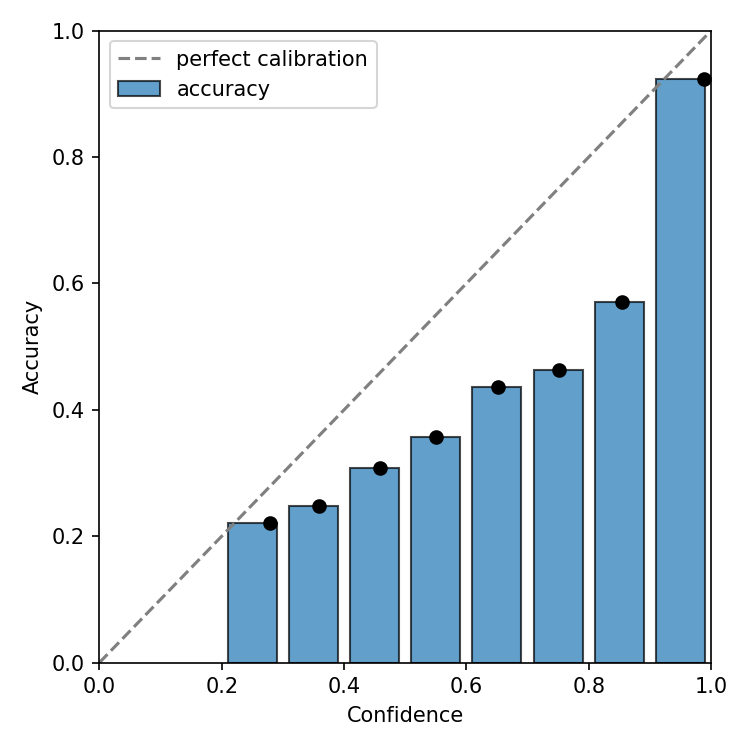
\includegraphics[width=\linewidth]{assets/bracs/tail_reliability_native.png}
    \caption{Severe, native assignment, tail classes}
  \end{subfigure}

  \vspace{0.8em}
  \begin{subfigure}[t]{0.48\linewidth}
    \centering
    
\includegraphics[width=\linewidth]{assets/bracs/tail_reliability_difficulty_aligned.png}
    \caption{Severe, aligned assignment, tail classes}
  \end{subfigure}\hfill
  \begin{subfigure}[t]{0.48\linewidth}
    \centering
    
\includegraphics[width=\linewidth]{assets/bracs/tail_reliability_difficulty_reversed.png}
    \caption{Severe, reversed assignment, tail classes}
  \end{subfigure}
  \caption{Reliability curves for the balanced reference and for the tail classes under the severe condition of each tail assignment, with bin accuracy against mean predicted confidence over ten equal-width bins, on the first locked partition.}
  \label{fig:reliability}
\end{figure}

\section{Per-Partition Results}
\label{app:splits}
The main text averages the three partitions with equal weight, which is only defensible if no single partition drives a conclusion. This appendix reports the cross-entropy deficits separately for each partition, alongside the spread of achieved severity across them.

\begingroup
\scriptsize
\resultstable{per_split}
\captionof{table}{Cross-entropy deficits by partition on both gate axes, with the equal-weight average and the relative achieved-severity spread across partitions, per condition and tail assignment.}
\label{tab:per-split}
\endgroup

\noindent No gate decision rests on a single partition, but the independent-support axis is the least uniform across them and this qualifies its reading. Its three units clear the \num{1.44}-percentage-point discrimination threshold in two of the three partitions and fall to \num{0.30}--\num{0.64} percentage points on the second, against \num{5.40}--\num{5.97} on the third; the equal-weight average that opens the gate is therefore carried by two partitions rather than three. On the nominal axis the pattern is steadier: every gate-passing unit clears the threshold in all three partitions except difficulty-aligned severe, whose smallest partition-level deficit is \num{1.19} percentage points. On the calibration axis the three balanced units are consistent in falling below threshold, and among the eight gate-passing units the reversed moderate condition is the most variable, ranging from \num{0.037}--\num{1.814} nats. Achieved severity itself varies across partitions by at most \num{0.002} in relative terms, well inside the \num{0.5} consistency guard.

The conclusions of Section~\ref{sec:rq2} are less exposed to this variation than the gate decisions are, because the recovery estimates on the independent-support axis are null in every partition rather than null only on average. The qualification attaches to the size of the independent-support deficit, not to the finding that nothing recovers it.

\section{Computational Cost}
\label{app:cost}
Cost bears on the design question because a method whose recovery requires substantially more computation than the reference is a different proposition from one that matches it. This appendix records processed examples, unique exposures, derived updates, examples per update, accelerator time, peak memory, and model size for every roster method, expressed as a matched difference against cross-entropy in the same condition.

\begin{landscape}
\begingroup
\scriptsize
\resultstable{cost}
\captionof{table}{Matched computational-cost comparisons against cross-entropy in the same condition, for every roster method and every recorded cost endpoint, with crossed patient-bootstrap intervals.}
\label{tab:cost}
\endgroup
\end{landscape}

\noindent The exposure budget is matched to within \num{0.6}\% across the roster, which is the property that makes the recovery comparison a comparison of methods rather than of data volume. Every method processes the same \num{503880} examples as cross-entropy to within rounding, except set learning, which exceeds it by \num{2727} to \num{2983} examples because its per-update example count depends on a tuned set size and the derived update count must be integral, and classifier retraining, which exceeds it by \num{129}. Post-hoc logit adjustment trains nothing of its own and reuses the cross-entropy checkpoint, so its processed-example difference is the full budget with a negative sign; its cost is a single pass to fit one scalar.

That matched exposure is achieved through unequal update counts, which is the intended trade. Set learning takes roughly \num{3800} fewer updates than cross-entropy at \num{641} more examples per update, and classifier retraining splits its budget between two stages in a fixed ratio. Accelerator time, peak memory, and parameter counts differ by amounts their intervals absorb in every case, so no roster method's recovery on this dataset is bought with materially more computation than the reference.

\clearpage
\bibliographystyle{plainnat}
\bibliography{references}

\end{document}
